\section{Research} \label{sec:research}

I would like to divide the work done in this project according to the front end and back end parts of the web application. 

\subsection{Front end}

For the front end of the application I explored various software to display the file structure of the repository as a graph and ways top make the graph interactive. Two main libraries I experimented with were three-force-graph \cite{threeforcegraph} and 3d-force-directed-graph \cite{3dforcegraph}.

Both libraries use a similar format for the data of the graph, which is a simple JSON file with the list of nodes and the links between the nodes.

\begin{lstlisting} [numbers=none]
{
    "nodes": [
        {
          "id": "1",
          "name": "A",
          "val": 1
        },
        {
          "id": "2",
          "name": "B",
          "val": 10
        },
        ...
    ],
    "links": [
        {
            "source": "1",
            "target": "2"
        },
        ...
    ]
}
\end{lstlisting}

My initial attempt was using the library three-force-graph \cite{threeforcegraph} , which arranged the directory tree on a plane. 

\begin{figure}[!htbp]
    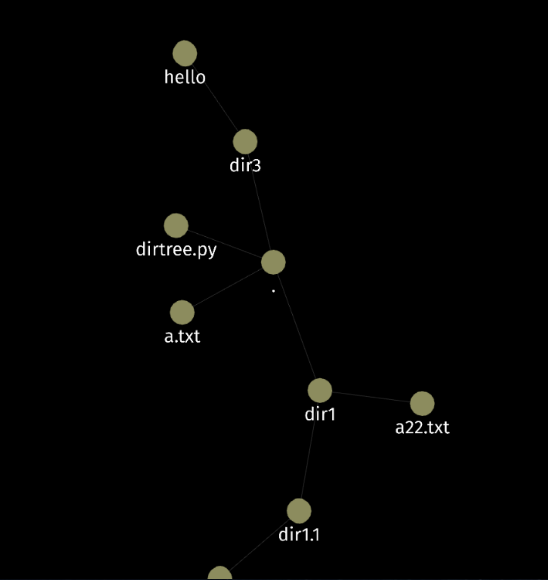
\includegraphics[width=8cm]{figs/three-force-graph_sample.png}
    \centering
    \caption{Directory Tree using Three-Force-Graph}
    \label{fig:three-force-graph}
\end{figure}

Figure \ref{fig:three-force-graph} shows an example of a small directory structure being displayed as a graph. While this works perfectly for small directorial structures, this is not the case for large directories as there would be an overcrowding of nodes. The 2D plane also fails to capture the idea of "levels" in a directory tree. Compared to this, the library \cite{3dforcegraph} created a 3D structure and also allowed the graph to be displayed as a DAG. This allowed the visualization of the levels in the directory tree as shown in figure \ref{fig:3d-force-directed-graph}

\begin{figure}[!htbp]
    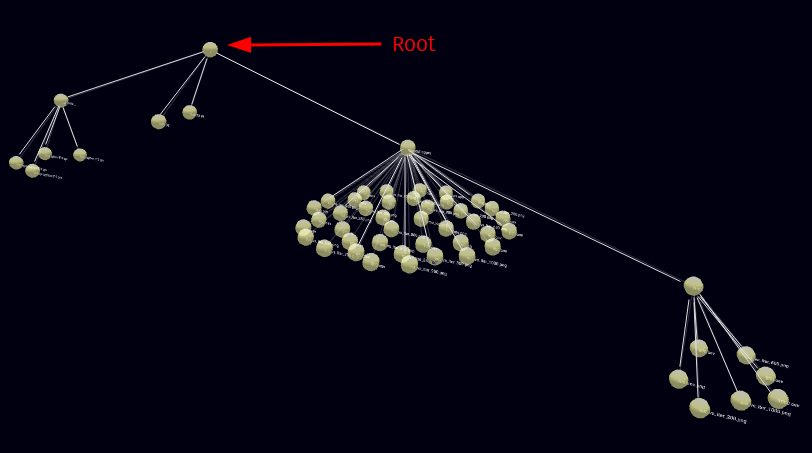
\includegraphics[width=8cm]{figs/3d-force-directed-graph_sample.png}
    \centering
    \caption{Directory Tree using 3d-force-directed-graph}
    \label{fig:3d-force-directed-graph}
\end{figure}

The next task was to try and load the graph for a large repository such as the Linux kernel \cite{linux}. As expected, this failed because of the size of the repository and rendering could not keep up with the amount of nodes and links. To overcome this we must dynamically load the data for parts of the tree that should be visible to the user. I experimented with two ways to provide the user a way to select parts of the tree they care about.

\begin{figure} [!htbp]
    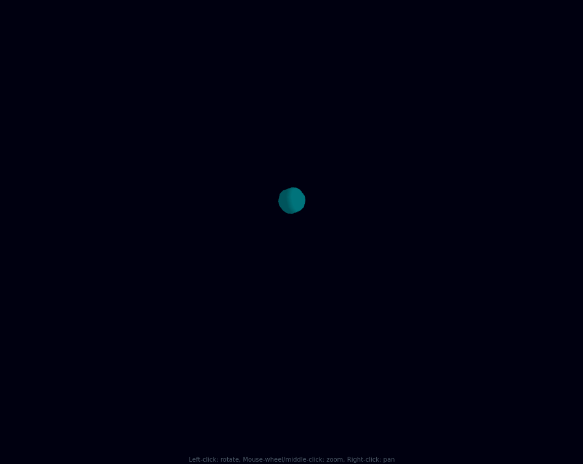
\includegraphics[width=4cm]{figs/node_click_0.png} \hfill
    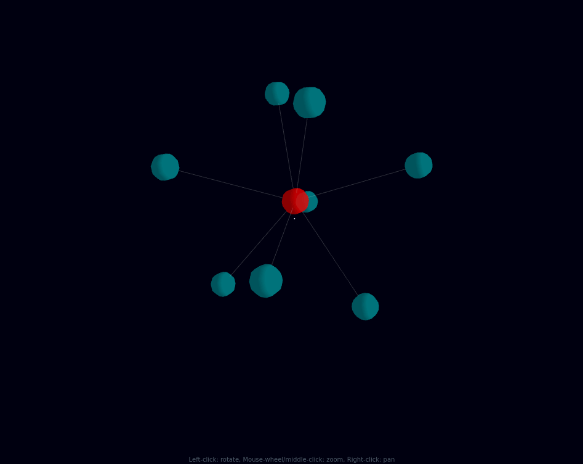
\includegraphics[width=4cm]{figs/node_click_1.png} \\
    \vspace{5mm}

    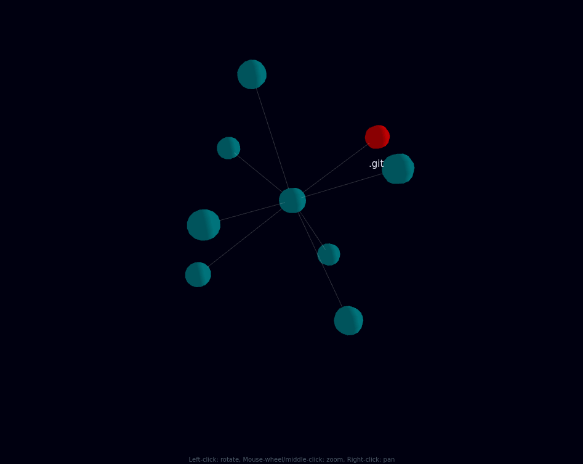
\includegraphics[width=4cm]{figs/node_click_2.png}\hfill
    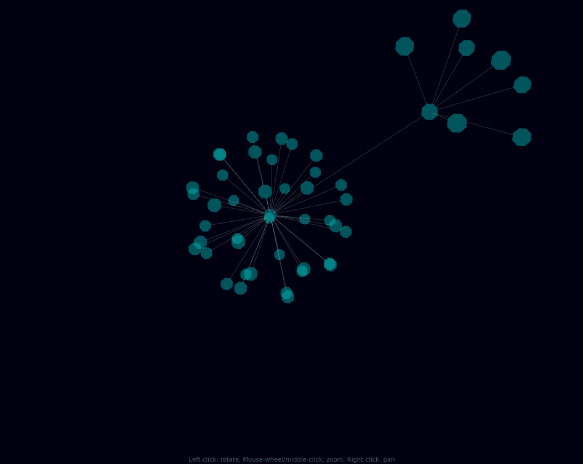
\includegraphics[width=4cm]{figs/node_click_3.png}
    \caption{ Node click and expansion mechanism}
    \label{fig:nodeclickmech}
\end{figure}

Figure \ref{fig:nodeclickmech} shows a mechanism that allows the user to click on the nodes to expand them and view the paths
to other files and directories. By doing this the application could avoid loading the entire graph and rendering slow downs. Although this method seems intuitive, it is time consuming as the user will have to manually expand all the nodes of the directories that they want to run a query for.

\begin{figure}[!htbp]
    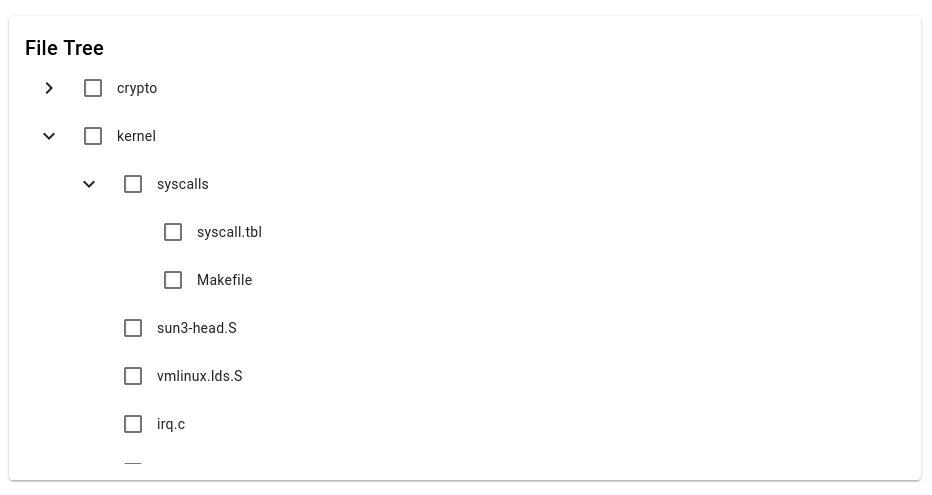
\includegraphics[width=8cm]{figs/file_tree.png}
    \centering
    \caption{File Tree}
    \label{fig:filetree}
\end{figure}

The second way to allow exploration of the graph was to use a file tree. Figure \ref{fig:filetree} shows an example of the Linux kernel file tree loaded. The file tree contains a check box next to each entry, which the user can check if the path to that directory or file should be visible in the graph.

\begin{figure} [!htbp]
    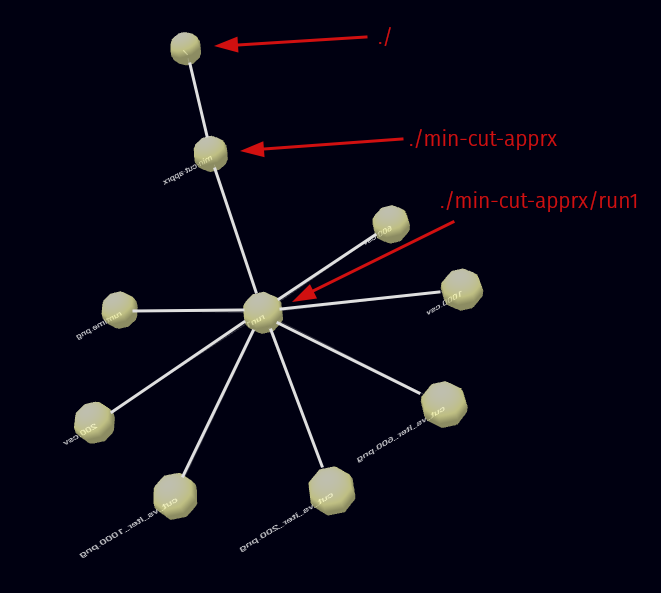
\includegraphics[width=4.5cm]{figs/file-tree-example.png} \hfill
    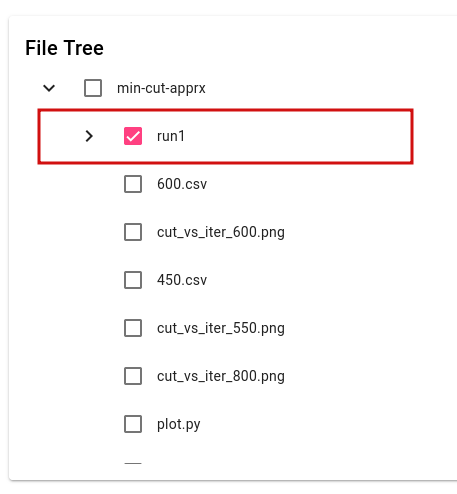
\includegraphics[width=4.5cm]{figs/file-tree-example2.png}
    \caption{ File Tree with Graph }
    \label{fig:filetreegraph}
\end{figure}

Figure \ref{fig:filetreegraph} shows an example where the "run" directory is selected in the file tree on the left. On the right in the figure, the user can see the path from the root to the "run" directory and also see the children of the selected directory. Using the file tree the user can select multiple paths they want to visualize and run queries on. For the UI such as the file tree, the application uses Angular Material \cite{angularmaterial}.
\subsection{Back end}

The back end uses a python Flask server that is also responsible for cloning the requested repository and generating the data required by the front end to visualize it. The server clones the file structure and runs a simple algorithm on the repository to generate the graph along the selected paths in the front end. The algorithm uses Depth First Search on the directory structure to traverse all the selected paths. It also works with wild card (*) entries in the path.

The server is also responsible for sending the complete file tree to the front end. The file tree is sent in the form of a JSON object after crawling the clones repository. Below is an example of the format of the data required to load the file tree into the front end:
\begin{lstlisting} [numbers=none]
{
    name: "dir1", 
    isFile: false, 
    path: "/dir1", 
    children: [
                {
                    name: "file1", 
                    isFile: true, 
                    path: "/dir1/file1", 
                    children: []
                },
                {
                    name: "dir2", 
                    isFile: false, 
                    path: "/dir1/dir2", 
                    children: [
                                {
                                    name: "file3", 
                                    isFile: true, 
                                    path: "/dir1/dir2/file3", 
                                    children: []
                                }  
                    ]
                }
            ]
}
\end{lstlisting}

Other work required by the back end which remains incomplete at the time of this report includes running the git queries. As mentioned previously, this can be achived by running the command line program git or using Github's REST API \cite{gitrestapi}. The idea is to allow the user to run queries from the front end and use colors to highlight the nodes affected by the results of that query. Here is a list of queries and corresponding commands for git that can be run by the user:
\begin{itemize}
    \item Query: List all branches in the repository, both local and remote.
    Command: \lstinline{git branch --all}

    \item Query: Find the most recent 10 commits that affected a specific file.
    Command: \lstinline{git log -n 10 -- <file_path>}

    \item Query: Show the commit history of a specific author.
    Command: \lstinline{git log --author="<author_name>"}
    
    \item Query: Display the commit history between two dates.
    Command: \lstinline{git log --since="<start_date>" --until="<end_date>"}
    
    \item Query: Show the changes introduced by a specific commit, including file modifications, additions, and deletions.
    Command: \lstinline{git show <commit_hash>}

    \item Query: Find commits containing a specific search term in the commit message.
    Command: \lstinline{git log --grep="<search_term>"}

    \item Query: Show the files that have changed between two branches.
    Command: \lstinline{git diff --name-status <branch1>..<branch2>}

    \item Query: Find the most changed files in the repository (by the number of lines changed).
    Command: \lstinline{git log --pretty=format: --name-only | sort | uniq -c | sort -rg}

    \item Query: Show the history of changes to a specific file, including the changes made in each commit, the author, and the commit message.
    Command: \lstinline{git log -p --follow -- <file_path>}

\end{itemize}